\documentclass{beamer}
\usepackage{hyperref} % URLs
\title[Critical Thinking]{Evaluating experiments (part 2)}
%\subtitle[short]{full}
\author{Andy J. Wills}
\date{\today}
\begin{document}

\frame{\titlepage}


\begin{frame}{Confounding variables}
	\begin{itemize}
        \item Any variable, other than the one you are attempting to
          study, that varies between conditions, and which could
          potentially have led to the effect you observe.
	\end{itemize}
\end{frame}

\begin{frame}{Confounds discussed so far...}
	\begin{itemize}
		\item Pre-existing differences (address by matching or randomization)
		\item Differential attrition (major issue, some partial solutions)
		\item Hawthorne effect / Placebo effect
		\item Demand charcteristics
	\end{itemize}
\end{frame}
		
\begin{frame}{Allocation of markers example}
\begin{itemize}
\item 300 students, 2 markers.
\item Marker 1 gets first 150 scripts handed in. Average mark B+
\item Marker 2 gets the rest. Average mark B.
\vspace{12 pt}
\item What might explain the difference between markers?
\end{itemize}
\end{frame}

\begin{frame}{Possible responses}
\begin{itemize}
\item Use a correlation analysis to study date-of-submission vs. grade relationship.
\item Randomize allocation of scripts to markers.
\end{itemize}
\end{frame}


\begin{frame}{Therapy example}
\begin{itemize}
\item Compare meditation-based therapy with relaxation training.
\item Large, randomized groups.
\item No pre-treatment differences in BDI
\item No differential attrition
\item BDI drops more for meditation than relaxation.
\item Meditation is the more effective treatment.
\end{itemize}
\end{frame}


\begin{frame}{Therapy example - Closer look}
\begin{itemize}
\item Compare meditation-based therapy with relaxation training.
\begin{itemize}
\item Meditation - Delivered by the people who developed the treatment
\item Relaxation - Delivered by people with no particular investment in relaxation therapy, who have been on a one-week training course in relaxation therapy.
\end{itemize}
\item Large, randomized groups.
\item No pre-treatment differences in BDI
\item BDI drops more for meditation than relaxation.
\item Meditation is the more effective treatment.
\end{itemize}
\end{frame}

\begin{frame}{Therapy example - Closer look}
\begin{itemize}
\item Compare meditation-based therapy with relaxation training.
\begin{itemize}
\item Meditation - Delivered by the people who developed the treatment
\item Relaxation - Delivered by people with no particular investment in relaxation therapy, who have been on a one-week training course in relaxation therapy.
\end{itemize}
\item Alternative explanation? - It's not the type of therapy that matters. It's some combination of therapist's belief in the treatment, their experience in delivering it, their general level of therapeutic expertise.
\end{itemize}
\end{frame}


\begin{frame}{Experimenter Effects - Data analysis - Example}
\begin{itemize}
\item Diary entries as a measure of happiness.
\item Participants write about their feelings
\item Experimenter rates for level of happiness.
\item If experimenter knows which condition the participant is in, this may bias their assessment of happiness.

\end{itemize}
\end{frame}


\begin{frame}{Experimenter Effects - Data analysis  }
\begin{itemize}
\item Objective measures immune? 
\item No! - Data analysis typically involves many decisions, all open to bias. 
\begin{itemize}
\item Should I exclude outliers?
\item If so, what's the cut-off?
\item Should I use a parametric or non-parametric test?
\item Are these tests multiple comparisons I should correct for, or separate analyses (for which I don't correct)?
\end{itemize}
\item If the experimenter knows which condition the participants are in, this could bias their decisions.
\end{itemize}
\end{frame}



\begin{frame}{Data analysis - Example }
\begin{itemize}
\item My theory predicts people react more quickly to auditory than to visual alarm signals.
\item I find this result if I exclude all reaction times above 3 seconds
\item But not if I keep all RTs
\item and not if I exclude all reaction times below 100ms.
\item I choose the 3 second cut-off
\item Am I sure that decision was unbiased?
\end{itemize}
\end{frame}


\begin{frame}{Blind testing}
\begin{itemize}
\item Single-blind testing - participant does not know which condition they are in. 
\begin{itemize}
\item e.g. Drug vs. placebo. Participants do not know which condition they are in. 
\end{itemize}
\item Double-blind testing - single-blind testing plus the experimenters do not know which condition is which until after they have completed their analysis.
\end{itemize}
\end{frame}


\begin{frame}{Order effects}
\begin{itemize}
\item Auditory versus visual alarm signals, within-subjects design
\item Visual (300ms) $\to$ Auditory (250ms)
\item Auditory faster?
\item Or, practice effect?
\end{itemize}
\end{frame}


\begin{frame}{Order effects}
\begin{itemize}
\item Auditory versus visual alarm signals, within-subjects design
\item Auditory (250ms) $\to$ Visual (300ms)
\item Auditory faster?
\item Or, fatigue effect?
\end{itemize}
\end{frame}



\begin{frame}{Order effects}
\begin{itemize}
\item Auditory versus visual alarm signals, within-subjects design
\item Randomly allocate participants to the two orders
\item Auditory (250ms) $\to$ Visual (300ms)
\item Visual (300ms) $\to$ Auditory (250ms)
\item Auditory faster - irrespective of order.
\item No practice or fatigue effect (mean RT across conditions 275 ms at time 1 and time 2).
\end{itemize}
\end{frame}



\begin{frame}{Difference versus no difference designs}
\begin{itemize}
\item The preferred hypothesis is that people differ in the speed with which they react to auditory and visual alarm signals.
\item The alternative theory against which this is compared is that there is no difference (nil hypothesis).
\item Problem - Experimental control is never perfect.
\item Thus - the nil hypothesis is almost certainly wrong, and detectably so if you test enough people.
\item Thus - the result of the study is known before you run it.
\item Thus - There was no point in running it.
\end{itemize}
\end{frame}


\begin{frame}{Better alternatives 1}
\begin{itemize}
\item One-tailed tests
\begin{itemize}
\item The preferred theory is that auditory is faster.
\item The alternative theory against which this is compared is that there is no difference (nil hypothesis).
\item If you find visual faster, you have disproved your theory.
\item So, whatever the result, there was a point to running this experiment (because the theory was falsifiable).
\end{itemize}
\end{itemize}
\end{frame}


\begin{frame}{Better alternatives 2}
\begin{itemize}
\item Ordinally different theories
\begin{itemize}
\item One well-established theory predicts that auditory is faster.
\item Another well-established theory predicts that visual is faster.
\item Whatever you find in this study, you've gained information (except in the unlikely case where the nil hypothesis was true).
\end{itemize}
\end{itemize}
\end{frame}


\begin{frame}{Better alternatives 3}
\begin{itemize}
\item Effect size
\begin{itemize}
\item Theory 1 - RT will differ between auditory and visual by more than two standard deviations.
\item Theory 2 - RT will differ between auditory and visual by less than two standard deviations.
\end{itemize}
\end{itemize}
\end{frame}



\begin{frame}{Statistical control myth}
\begin{itemize}
\item The idea you can ``control for'' group differences by clever statistics (e.g. Analysis of Covariance).
\item Example
\begin{itemize}
\item Group 1 - Depressed. Selected on BDI score
\item Group 2 - Nondepressed. Selected on BDI score.
\item Group 1 are worse than Group 2 on a memory test
\end{itemize}
\item Depression causes poor memory? Poor memory causes depression?
\item Inspection reveals Group 1 are, on average, older than Group 2. 
\item Perhaps age is the causal factor?
\item The Myth - you can ``control for'' age as a factor by entering as a co-variate into your analysis.
\item This is false (Miller \& Chapman, 2001). 
\end{itemize}
\end{frame}


\begin{frame}{Infallible Flowchart of Paper Evaluation}
\begin{enumerate}
\item \textbf{Central topic} (What is it about?)
\item \textbf{Central research question} (What do they wish to test?)
\item \textbf{Central rationale} (Why bother?)
\item \textbf{Essence of Method} (How did they test their question?)
\item \textbf{Key Result}
\item \textbf{Central Valid Conclusion}
\end{enumerate}
\end{frame}



\begin{frame}{Evaluating a research paper}

\centerline{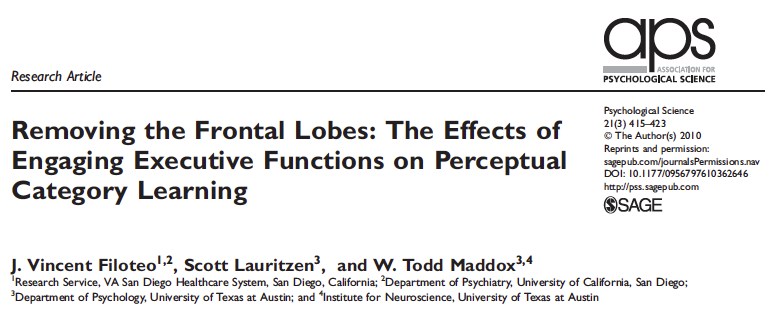
\includegraphics[width=1\textwidth]{filoteo.png}}

\end{frame}


\begin{frame}{Central topic}

\centerline{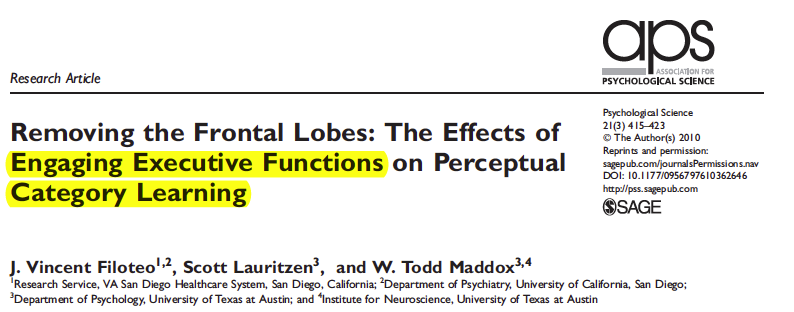
\includegraphics[width=1\textwidth]{filoteo2.png}}


\begin{itemize}
\item Category learning - The act of learning how to divide the world into groups of things.
\item Executive function - Management of cognitive processes.
\end{itemize}

\end{frame}



\begin{frame}{Research question}

\centerline{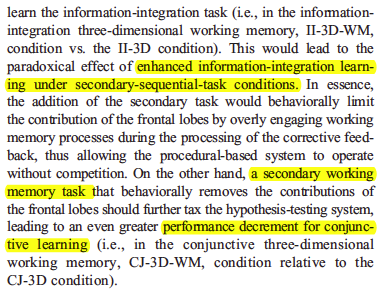
\includegraphics[width=.9\textwidth]{filoteoendintro.png}}
\tiny (c) 2010. J.V. Filoteo, S. Lauritzen, W.T. Maddox. 
\end{frame}



\begin{frame}{Research question}

\centerline{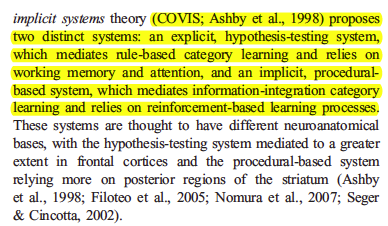
\includegraphics[width=.9\textwidth]{filoteotheory.png}}
\tiny (c) 2010. J.V. Filoteo, S. Lauritzen, W.T. Maddox. 
\end{frame}



\begin{frame}{Methodology - Key questions}

\begin{itemize}
\item What is the dependent variable (DV)? 
\item Is the DV appropriate for the question?
\item What are the independent variables (IV)?
\item Are the IVs appropriate for the question?
\item Are the IVs confounded with any other variables?
\end{itemize}

\end{frame}



\begin{frame}{DV and IVs}

\centerline{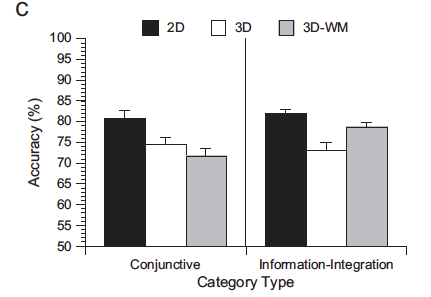
\includegraphics[width=0.5\textwidth]{filoresults.png}}

\begin{itemize}
\item DV - Accuracy. Appropriate.
\item IV1 - Category type (conjunctive vs. information integration). Appropriate.
\item IV2 - Cognitive load (digit load vs. no digit load). Appropriate.
\end{itemize}

\tiny Image (c) 2010. J.V. Filoteo, S. Lauritzen, W.T. Maddox.

\end{frame}



\begin{frame}{IV confound}

\centerline{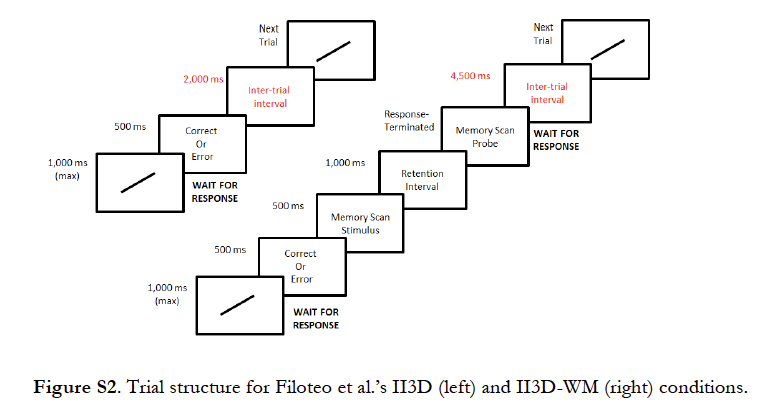
\includegraphics[width=1.2\textwidth]{filomistake.png}}

\tiny(c) 2013. Newell, Moore, Milton \& Wills

\end{frame}

\begin{frame}{Key Result}

\centerline{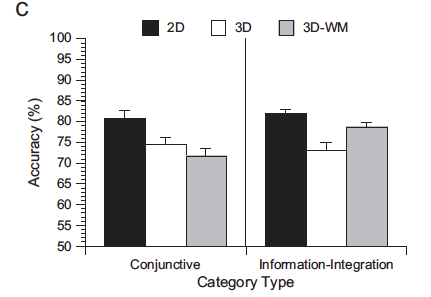
\includegraphics[width=0.5\textwidth]{filoresults.png}}

\begin{itemize}
\item Concurrent load increases accuracy for II structure.
\item Concurrent load decreases accuracy for CJ structure.  

\end{itemize}

\end{frame}

\begin{frame}{Infallible Flowchart of Paper Evaluation}
\begin{itemize}
\item \textbf{Central topic} (What is it about?)
	
  Effect of ``engaging'' executive functions on category learning
\item \textbf{Central research question} (What do they wish to test?)
	
  Secondary task will improve information-integration category
  learning but hurt conjunctive category learning.
\item \textbf{Central rationale} (Why bother?)
	 
	 Prediction of COVIS theory
\end{itemize}
\end{frame}

\begin{frame}{Infallible Flowchart of Paper Evaluation}
\begin{itemize}

\item \textbf{Essence of Method} (How did they test their question?)
	 
  DV - Accuracy. IV1 - category structure (CJ vs. II). IV2 - digit
  load (present vs. absent).  IV2 confounded with ITI.  The Method is
  not a particularly good test of the central research question.
\item \textbf{Key Result}
	 
	 Digit load increases accuracy in II.
	 Digit load has no significant effect in CJ.
	 These two conditions differ significantly. 
	 The results are partially consistent with the hypothesis.
\item \textbf{Central Valid Conclusion}
	
  Digit load, combined with extra time to think, improves accuracy on
  an information integration category structure.
\end{itemize}

\tiny Except where noted, this work is licensed under a Creative
Commons Attribution-ShareAlike 4.0 International Licence. Last update:
\today

\end{frame}




\end{document}

%%% Local Variables:
%%% mode: latex
%%% TeX-master: t
%%% End:
